\begin{quotation}\itshape
``Brand new LP just dropped!''
\end{quotation}

Over your previous years and courses, you have seen a range of powerful algorithm design techniques with which to attack algorithmic problems. Once you have formulated the task you want to solve, you have by now an array of tools to try and solve it: greedy algorithms, divide-and-conquer, dynamic programming\dots Linear Programming (LP for short) is another one, very powerful. We will only scratch the surface here, but what it does is quite simple to state:
\begin{framed}
    Maximize a linear function subject to linear inequality constraints on variables $x_1,\dots, x_\ns$ of interest.
\end{framed}
In its most general form, this can be rephrased as follows:\marginnote{You can do minimisation tasks instead of maximisation, of course. Can you see how?}
\begin{align*}
    \operatorname{maximise}\ &\purple{c}^\transp x\\
    \text{subject to}\  &\red{A}x \leq \green{b}
    &x \geq 0
\end{align*}
where the inequalities are to be taken coordinate-wise; $x\in\R^{\ns}$ is the set of variables (encoding the solution), and $\purple{c}\in\R^{\ns}$, $\red{A}\in \R^{\green{m}\times \ns}$, and $\green{b}\in\R^{\green{m}}$ encode the task to be solved: $\purple{c}$ the objective function, and $\red{A},\green{b}$ the constraints. This may look a little daunting in this form, so here is a less compressed version:
\begin{align*}
    \operatorname{maximise}\ \sum_{i=1}^{\ns}& \purple{c}_i x_i\\
    \text{subject to}\qquad&  \\
    \sum_{i=1}^{\ns}\red{A}_{ji} x_i &\leq \green{b}_j, \qquad 1\leq j\leq \green{m}\\
    x_i &\geq 0, ~\qquad 1\leq i\leq \ns\\
\end{align*}
We will see examples through the chapter, but here are the key things to keep in mind regarding Linear Programming:
\begin{framed}
\begin{itemize}
    \item LP is \textsf{P}-complete: every problem that has a polynomial-time algorithm can be solved by (some) linear program.
    \item LPs can be solved efficiently \emph{in theory}: every linear program can be solved (to arbitrary precision) in time polynomial in $\ns,\green{m}$ (or, more precisely, in the size of the representation of $\red{A},\green{b},\purple{c}$, and desired accuracy.)
    \item LPs can be solved efficiently \emph{in practice}: there are actual algorithms which solve LPs very quickly, and you can use them.
    \item There is a \emph{very rich theory} on Linear Programming, enough to fill a whole course: we will not touch on most of it.
\end{itemize}
\end{framed}\marginnote{\vspace{-7em}\\For instance, \textsc{COMP4530/5530}: Discrete Optimisation. Consider taking that course!}
So, for the rest of this chapter, whenever we end up with an LP (on a polynomial number of variables $\ns$ and constraints $\green{m}$), we will simply wave a magic wand and say ``this can be efficiently solved to get an optimal solution,'' without caring too much about \emph{how}.\medskip 

LPs are very powerful, and a wonderful arrow in our algorithmic quiver, allowing us in principle to solve in a systematic way every problem in \textsf{P}.\footnote{This is not saying we \emph{should}. There may be faster algorithms than writing and solving the corresponding LP!}  The issue, of course, is that often we want to solve problems that are \emph{not} known to be in \textsf{P}: problems which, by definition, we do not know how to express as an LP with a polynomial number of variables and constraints. But we would still like to solve these approximately! \emph{Can LPs still help somehow?}

Specifically, as in the chapter on streaming (but for different reasons), given a hard computational task $\mathcal{T}$ we would like to obtain an $\purple{\alpha}$-approximation to an optimal solution to $\mathcal{T}$, for some approximation factor $0 < \purple{\alpha}\leq 1$: that is, giving an instance $I$ of $\mathcal{T}$, we want to output a solution $S=S(I)$ whose value satisfies\marginnote{For maximisation problems. For minimisation, that would be $\opt(I) \leq \val(S) \leq \purple{\alpha}\cdot \opt(I)$, for $\purple{\alpha} \geq 1$.}
\begin{equation}
    \purple{\alpha} \cdot \opt(I) \leq \val(S) \leq \opt(I)
\end{equation}
(with high probability, or in expectation, if our algorithm is randomised), where $\opt(I)$ denotes the optimal value: the best achievable by any solution for instance $I$.

\subsection{Let's forget about LPs.} One standard approach is to first, essentially, shrug and formulate our problem as something which is \emph{not} an LP, but instead includes some stronger constraints that are not linear. That is, instead of constraints on our variables like $x_i \geq 0$ we allow constraints of the form ``$x_i$ must be an integer.'' (Most often, $x_i \in\{0,1\}$.) 

Here is an example, for a problem that is, actually, in \textsf{P}, one we have seen before: $st$-\textsc{Min-CUT}.
\begin{figure}[htbp!]
\begin{align*}
    \operatorname{maximise}\ -\sum_{e\in E}& c_ex_e\\
    \text{subject to}\qquad&  \\
    y_s &= 0\\
    y_t &= 1\\
    y_v &\leq y_u + x_e, \qquad \forall e=(u,v)\in E\\
    \color{red}x_e, y_v &\color{red}\in \{0,1\}\qquad \forall e\in E, v\in V
\end{align*}
\caption{\textsc{Min-CUT}, on an directed graph $G=(V,E)$ with edge weights $c\colon E\to \R_+$ and source and sink vertices $s,t\in V$, formulated as an ILP.}
\end{figure}
To interpret this: we have $|\red{V}|+|\orange{E}|$ variables. The $x_e$'s indicate whether edge $e$ is part of the cut, while the $y_v$'s indicate whether vertex $v$ is in the same connected component as the sink $t$. The goal is to select values for the variables in order to minimise the weight of the cut, $\sum_{e\in E} c_ex_e$. 
So if we could solve this optimally, we would have a solution to our $st$-\textsc{Min-CUT} instance!\smallskip

As we will see, switching from LPs to ILPs comes at a significant advantage: we can encode many more problems as Integer Linear Programs (ILPs)\marginnote{Integer Linear Program (ILP)}, including \textsf{NP-Hard} ones. This also comes at a significant cost: contrary to LPs, we just don't know how to solve ILPs efficiently in general!

So \emph{what is the point of all this?} We know how to solve LPs very fast, but they may not capture the problems we care to solve. ILPs might, but we don't know how to solve them efficiently. This is even more dire given the example above: we \emph{have} very efficient algorithms for $st$-\textsc{Min-CUT}. But now that we formulated \textsc{Min-CUT} as an ILP, we just\dots don't know how to solve it that way?

\subsection{Let's not forget about LPs.} Here comes the key insight: once we have formulated a problem as an ILP, we can \emph{relax}\marginnote{``LP Relaxation''} its constraints to convert it into an LP \emph{which we then can solve efficiently}. This gives us a solution to a different problem (since we changed the constraints), but sometimes, if we are lucky, from this solution to the \emph{relaxed} problem we can extract a solution to the \emph{original} problem, and still can say something interesting about its value (quality).

Relaxing the problem basically means converting all the ``hard'' integer constraints into continuous, linear ones: \eg for the~\textsc{Min-CUT} problem, relaxing the ILP above yields the LP given in~\cref{fig:lp:relax:mincut}.
\begin{figure}[htbp]
\begin{align*}
    \operatorname{maximise}\ -\sum_{e\in E}& c_ex_e\\
    \text{subject to}\qquad&  \\
    y_s &= 0\\
    y_t &= 1\\
    y_v &\leq y_u + x_e, \qquad \forall e=(u,v)\in E\\
    \color{blue}x_e, y_v &\color{blue}\in [0,1]\qquad \forall e\in E, v\in V
\end{align*}
\caption{The LP relaxation to the previous \textsc{Min-CUT} ILP relaxation.}\label{fig:lp:relax:mincut}
\end{figure}
We can then solve this, giving us a solution $S_{\rm{} LP}$ to our problem. We then have the nice, ``obvious'' fact:
\begin{fact}
    \label{fact:lpilp}
    Let $\opt_{\rm ILP}$ be the optimal value of a solution to an ILP (maximisation problem), and $\opt_{\rm LP}$ be the optimal value of a solution to its LP relaxation. Then
    \[
    \opt_{\rm ILP} \leq \opt_{\rm LP}\,.
    \]
    (For a minimisation problem, the inequality is reversed.)
\end{fact}



Of course, this will not in general be a solution to the original problem (here, $st$-\textsc{Min-CUT}), because, well, what does it mean for a vertex to have $y_v=0.5786$? Which side of the cut is vertex $v$?

\paragraph{Rounding!} The next key insight is that we can often \emph{extract} a solution to the ILP from the (optimal) solution to the LP. Now, we will have to lose something in the process\marginnote{Otherwise, we would know how to solve the ILP! Possibly proving \textsf{P}=\textsf{NP} along the way.}: either the solution is only a valid solution with high probability (with small probability, some of the constraints will be violated), or the value of the resulting solution is not quite optimal. Here, we will focus on the latter. Going back to our \textsc{Min-CUT} example: we solved the LP relaxation, getting an optimal solution
\[
    (x^\ast, y^\ast) \in [0,1]^{|\orange{E}|+|\red{V}|}
\]
to the LP, with value $\opt_{\rm LP}$. We want to get a valid solution to our graph problem, so getting a solution $y \in \{0,1\}^{|\red{V}|}$ from this for which, hopefully, $\val(y) \approx \opt_{\rm LP}$.

A very natural idea: let's \emph{round the coordinates} of $y^\ast$! Rounding things in $[0,1]$ will give us things in $\{0,1\}$, and that seems to fit the bill. This works for \emph{some} problems, and is called \emph{deterministic rounding}. The hard part, however, is then to be able to argue anything about $\val(y)$: for \textsc{Min-CUT} for instance, if all coordinates of $y^\ast$ are say 0.50001 (except of course $y_s$), then we round them all to $1$, and we include \emph{all} vertices except $s$ in our cut. Maybe not a good idea.\marginnote{Check your understanding: why are we looking at $y$, and not $x$ (say, setting $x_e$ to $1$ with probability $x^\ast_e$)?}

But what about \emph{randomised} rounding then? One issue with the above rounding is that we had a \emph{deterministic} threshold, $1/2$, which did not allow us to say much about the result, and in particular did not let us leverage any guarantee provided by the LP we just solved. So, deterministic threshold: not very useful. Maybe we can pick our threshold \emph{randomly} then?
\begin{algorithm}[H]
\begin{algorithmic}[1]
    \State Pick $\tau$ in $(0,1)$ uniformly at random.
    \ForAll{$v\in \red{V}$}
        \State Set $y_v=1$ if $y^\ast_v > \tau$, $0$ otherwise
    \EndFor
    \State \Return $y$.
\end{algorithmic}
\caption{Randomised rounding for the LP relaxation of \textsc{Min-CUT}.\label{algo:random:rounding:mincut}}
\end{algorithm}
That's all. \emph{Does it work?} Clearly, this returns a valid cut, as $y \in \{0,1\}^{|\red{V}|}$ with $y_s = 0$, $y_t=1$. Can we say anything about the (expected) value of the ? As it turns out, yes! Using the LP we solved as a guide.
\begin{theorem}
    The cut $y$ returned by~\cref{algo:random:rounding:mincut} satisfies $\expect{\val(y)} = \opt_{\rm ILP}.$
\end{theorem}
\begin{proof}
    By linearity of expectation,
    \begin{align*}
    \expect{\val(y)}
    &= \sum_{e\in E} c_e \expect{\indicSet{e \text{ is cut}}}
    = \sum_{e=(u,v)\in E} c_e \probaOf{y_u = 0, y_v = 1}
    \end{align*}
    We want to relate this to $\sum_{e\in E} c_e x^\ast_e$, since this is what we know is the optimal value of the LP. But, for any $e=(u,v)\in E$, using the third constraint of the LP, $y_v - y_u \leq x^\ast_e$, and so
    \[
        \probaOf{y_u = 0, y_v = 1}
        = \probaOf{y^\ast_u \leq \tau < y^\ast_v}
        \leq x^\ast_e
    \]
    from which 
    \begin{align*}
    \expect{\val(y)}
    &\leq \sum_{e=(u,v)\in E} c_e x^\ast_e = -\opt_{{}LP} \leq -\opt_{\rm{}ILP}
    \end{align*}
    the last inequality from~\cref{fact:lpilp}. In expectation, the solution we get is at least as good as the minimum cut value: since it cannot be \emph{better} (no valid cut can be better than the minimum cut!), it \emph{is} the minimum cut value.
\end{proof}

This is nice! But we used a big hammer (ILP, LP relaxation, then randomised rounding) in order to solve a problem we already knew how to solve deterministically \emph{via} Max-Flow, and it's not even clear the new approach is faster. This was very good for the sake of illustrating the ideas, but \emph{surely}, there has to be more compelling? To see one, let us turn to a \emph{bona fide} \textsf{NP-Hard} problem, \textsc{Max-SAT}.

\section{Approximation algorithm for \textsc{Max-SAT}} In the \emph{maximum satisfiability problem}  (\textsc{Max-SAT}), we have $\ns$ Boolean variables $x_1,\dots, x_\ns\in\{0,1\}$, grouped into $\green{m}$ \emph{clauses} $C_1,\dots, C_{\green{m}}$. Each clause is a \emph{disjunction} of the variables, that is, of the form
\[
    C_j = x_{i_1}\lor \lnot x_{i_2}\lor \dots \lor x_{i_\ell}
\]
(a logical \textsf{OR} of \emph{literals}, where a literal is either a variable $x_i$ or its negation $\lnot x_i$). A clause is \emph{satisfied} if it evaluates to $1$, that is, if at least one of the literals in the clause is $1$. The \textsc{Max-SAT} problem asks, given such a formula $\phi= (C_1,\dots, C_{\green{m}})$, to assign values to all $\ns$ variables in order to maximise the number of satisfied clauses, \ie \marginnote{All we are going to talk about generalises to the weighted version, where clause $C_j$ has a weight $w_j\geq 0$ and the goal is to maximise $\sum_{j=1}^{\green{m}} w_j \indic{C_j \text{ is satisfied}}$. Check it!}
\[
    \val_\phi(x_1,\dots, x_\ns) = \sum_{j=1}^{\green{m}} \indicSet{C_j \text{ is satisfied}}
\]
Without loss of generality, we assume that (1)~all $\green{m}$ clauses are distinct, (2)~$x_i$ and $\lnot x_{i}$ do not appear both in any given clause (as this makes it automatically satisfied), and (3)~each literal appears at most once in each clause (no repetition, as they are useless). The \emph{length} of a clause $C_j$ is the number of literals in the clause, denoted $\ell_j = |C_j|$.
\begin{fact}
    \textsc{Max-SAT} is \textsf{NP-Hard}. (Even deciding whether $\opt(\phi) = \green{m}$ is \textsf{NP-Complete}.)
\end{fact}
But can we \emph{approximate} $\opt(\phi)$? As it turns out, getting \emph{some} approximation is not too difficult:
\begin{theorem}
    \label{theo:randomised:maxsat}
    The ``obvious'' randomised algorithm which sets each variable $x_i$ independently and uniformly at random gives, in expectation, a $\frac{1}{2}$-approximation for \textsc{Max-SAT}.
\end{theorem}
\begin{proof}
    Consider a fixed clause $C_j$. The probability that $C_j$ is \emph{not} satisfied is the probability to set every single one of the $\ell_j$ literals the wrong way, which is
    \[
        \frac{1}{2^{\ell_j}}
    \]
    and so, by linearity of expectation, and as $\ell_j \geq 1$ for all $1\leq j\leq \green{m}$,
    \begin{align}
    \expect{\val_{\phi}(x)} = \sum_{j=1}^{\green{m}} \Paren{1-\frac{1}{2^{\ell_j}}} \geq \frac{1}{2}\green{m} \geq \frac{1}{2}\opt(\phi)\,. \label{eq:intermediate:naiverandomised}
    \end{align}
    proving the result.
\end{proof}
Interestingly, one nice feature is that this gives a better guarantee for ``long clauses'', those for which $\ell_j \geq 2$. For instance, for \textsc{Max-E3SAT}, where each clause has \emph{exactly} 3 literals, we get a $\frac{7}{8}$-approximation (since $1-{1}/{2^{\ell_j}} = \frac{7}{8}$ for every $j$)! 

Again, this is fine, but (1)~a $(1/2)$-approximation is not that exciting, and (2)~there is no LP in there! Now that the warmup is over, let us formulate \textsc{Max-SAT} as an ILP. Besides the $\ns$ variables $y_1,\dots, y_{\ns}$ (corresponding directly to the $\ns$ Boolean variables $x_1,\dots, x_{\ns}$), we will have $\green{m}$ additional variables, one per clause, where $z_j$ indicates whether $C_j$ is satisfied:
\begin{figure}[htbp!]
\begin{align*}
    \operatorname{maximise}\ \sum_{j=1}^{\green{m}}&\ z_j\\
    \text{subject to}\qquad&  \\
    \sum_{i: x_i \in C_j} &y_i + \sum_{i: \lnot x_i \in C_j} (1-y_i) \geq z_j \qquad ~\forall 1\leq j\leq \green{m}\\
    \color{red}y_i &\color{red}\in \{0,1\}
    \quad\quad\qquad\qquad\qquad\quad  \forall 1\leq i\leq \ns\\
    \color{red}z_j &\color{red}\in \{0,1\}
    \quad\quad\qquad\qquad\qquad\quad \forall 1\leq j\leq m
\end{align*}
\caption{\textsc{Max-SAT}, formulated as an ILP.}
\end{figure}
We then need to show the following:
\begin{lemma}
    The optimal value of the ILP is equal to $\opt(\phi)$.
\end{lemma}
\begin{proof}[Sketch.]
    To check: if $x\in\{0,1\}^\ns$ is an optimal solution to the \textsc{Max-SAT} problem on input $\phi=(C_1,\dots, C_{\green{m}})$, then one can extract from it a valid solution to the ILP, with the same value. Conversely, from an optimal solution to the ILP, one can obtain a solution to \textsc{Max-SAT} with the same value.
\end{proof}
As before, we don't know how to solve this: so we go for the LP relaxation.
\begin{figure}[htbp!]
\begin{align*}
    \operatorname{maximise}\ \sum_{j=1}^{\green{m}}&\ z_j\\
    \text{subject to}\qquad&  \\
    \sum_{i: x_i \in C_j} &y_i + \sum_{i: \lnot x_i \in C_j} (1-y_i) \geq z_j \qquad ~\forall 1\leq j\leq \green{m}\\
    \color{blue}0\leq y_i &\color{blue}\leq 1
    \quad\quad\qquad\qquad\qquad\qquad\quad  \forall 1\leq i\leq n\\
    \color{blue}0\leq z_j &\color{blue}\leq 1
    \quad\quad\qquad\qquad\qquad\qquad\quad \forall 1\leq j\leq m
\end{align*}
\caption{\textsc{Max-SAT}, LP relaxation to the above ILP.\label{alg:maxsat:lp:relax}}
\end{figure}
After solving (optimally) this LP relaxation in time polynomial in $\ns$ and $\green{m}$, we get a solution $y^\ast,z^\ast$ optimal for this LP. How do we round this to get a (valid) solution $x$ for the ILP (equivalently, for \textsc{Max-SAT}) about which we can prove something? Here's another key idea: we want values $x_i\in \{0,1\}$ but we are given $y_i\in[0,1]$. The good thing is, there is a very natural interpretation to values in $[0,1]$: seeing them as \emph{probabilities}. This suggests the following randomised rounding scheme:
\begin{algorithm}[H]
\begin{algorithmic}[1]
    \Require Instance $\phi=(C_1,\dots,C_{\green{m}})$ of \textsc{Max-SAT} on $\ns$ variables
    \State Solve the LP relaxation (\cref{alg:maxsat:lp:relax}), getting solution $(y^\ast,z^\ast)$.
    \ForAll{$1\leq i\leq \ns$}
        \State Set $x_i = 1$ with probability $y^\ast_i$, independently of others.
    \EndFor
    \State \Return $x$.
\end{algorithmic}
    \caption{Randomised rounding of the LP relaxation for \textsc{Max-SAT}.\label{alg:randomrounding:maxsat}}
\end{algorithm}
This is quite simple, and produces a valid assignment of the Boolean variables $x_1,\dots, x_{\ns}$. How well does it fare in terms of clauses satisfied? As it turns out, not badly at all!
\begin{theorem}
    \label{theo:randomrounding:maxsat}
    The randomised rounding given in~\cref{alg:randomrounding:maxsat} gives, in expectation, a $(1-\frac{1}{e})$-approximation for \textsc{Max-SAT}.\marginnote{$1-1/e\approx 0.632$: better than $1/2$!}
\end{theorem}
\begin{proof}
    As before, we need to use what the LP we solved did, as a guide to analyse the expected value of our solution. What we can write is
    \begin{align*}
        \expect{\val_\phi(x)} 
        &= \sum_{j=1}^{\green{m}}\probaOf{C_j \text{ satisfied}} 
        = \sum_{j=1}^{\green{m}} \Paren{1-\probaOf{C_j \text{ not satisfied}}}
    \end{align*}
    By independence of our assignments of the $x_i$'s, and since each variable appears (negated or not) at most once per clause, we also have that, for every $j$,
    \begin{align}
    \probaOf{C_j \text{ not satisfied}}
    &= \prod_{i: x_i \in C_j} \probaOf{x_i=0}\cdot \prod_{i: \lnot x_i \in C_j} \probaOf{x_i=1} \notag\\
    &= \prod_{i: x_i \in C_j} (1-y^\ast_i)\cdot \prod_{i: \lnot x_i \in C_j} y^\ast_i \label{eq:before:amgm}
    \end{align}
    This is a product, but what the LP gives us a handle on is a sum: from the constraints, what we know is that, for every $j$,
    \[
    \sum_{i: x_i \in C_j} y_i + \sum_{i: \lnot x_i \in C_j} (1-y_i) \geq z_j
    \]
    To relate products to sums (or, rather, to averages), one very handy tool is the  \emph{inequality of arithmetic and geometric means} (AM--GM inequality):   \marginnote{Another life-saver: the AM--GM inequality.}
    \begin{fact}
        \label{fact:am:gm}
        For any $a_1,\dots,a_k \geq 0$, 
        \[
        \sqrt[k]{a_1 a_2\cdots a_k} \leq \frac{a_1+a_2+\dots + a_k}{k}
        \]
    \end{fact}
    Applying this to~\eqref{eq:before:amgm} gives us
    \begin{align*}
    \probaOf{C_j \text{ not satisfied}}
    &= \prod_{i: x_i \in C_j} (1-y^\ast_i)\cdot \prod_{i: \lnot x_i \in C_j} y^\ast_i \\
    &\leq \Paren{ \frac{\sum_{i: x_i \in C_j} (1-y^\ast_i) + \sum_{i: \lnot x_i \in C_j} y^\ast_i}{\ell_j}  }^{\ell_j} \\
    &=\Paren{ 1-\frac{\sum_{i: x_i \in C_j} y^\ast_i + \sum_{i: \lnot x_i \in C_j} (1-y^\ast_i)}{\ell_j}  }^{\ell_j} \\
    &\leq \Paren{ 1-\frac{z^\ast_j}{\ell_j}}^{\ell_j} \tag{By the LP constraint}
    \end{align*}
    and so, recalling where we came from,
    \begin{align}
        \expect{\val_\phi(x)} 
        &\geq \sum_{j=1}^{\green{m}} \Paren{1-\Paren{ 1-\frac{z^\ast_j}{\ell_j}}^{\ell_j}}
    \end{align}
    We are almost there! We want to relate this to what we \emph{know} is the optimal value of the LP, $\sum_{j=1}^{\green{m}} z^\ast_j$. To do so, observe that for any $\ell\geq 1$ the function
    \[
    f(z) = 1-\Paren{1-\frac{z}{\ell}}^\ell, \qquad z\in [0,1]
    \]
    is concave, and as a result is above its linear interpolation (see~\cref{fig:randomrounding:concave}):\marginnote{Exercise: prove it!}
    \[
        f(z) \geq \Paren{1-\Paren{1-\frac{1}{\ell}}^\ell} z, \qquad z\in [0,1]
    \]
    \begin{figure}[htbp]
        \centering
        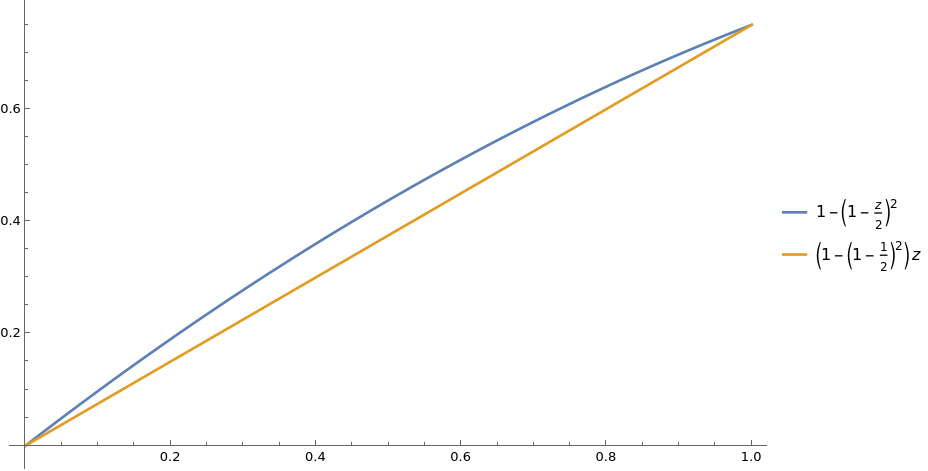
\includegraphics[width=1.25\textwidth]{figures/fig-randomrounding-concaveconcave.png}
        \caption{An illustration of the inequality for $\ell=2$.}
        \label{fig:randomrounding:concave}
    \end{figure}
    Using this, we finally get\marginnote{We invoke the ``fact'' that 
    \[
    \sup_{\ell \geq 1}\Paren{ 1-\frac{1}{\ell_j}}^{\ell_j} = 1/e\,.
    \]
    }
        \begin{align}
        \expect{\val_\phi(x)} 
        &\geq \sum_{j=1}^{\green{m}} \Paren{1-\Paren{ 1-\frac{1}{\ell_j}}^{\ell_j}}\cdot z^\ast_j \label{eq:intermediate:rounding:guarantee}\\
        &\geq \inf_{\ell \geq 1}\Paren{1-\Paren{ 1-\frac{1}{\ell}}^{\ell}}  \cdot \sum_{j=1}^{\green{m}} z^\ast_j \notag\\
        &= \Paren{1-\frac{1}{e}} \opt_{\rm LP} \notag\\
        &\geq \Paren{1-\frac{1}{e}} \opt_{\rm ILP} \notag
    \end{align}
    concluding the proof.
\end{proof}

\paragraph{Are we done?} We started by showing a simple randomised approach giving an expected $1/2$-approximation to \textsc{Max-SAT}. By spending more time, effort, and relaxing (an ILP), we obtained an efficient randomised algorithm, less simple but giving a better guarantee: an expected $0.632$-approximation. \emph{Can we do better?}

Surprisingly, yes: we can get a $3/4$-approximation, by combining the two! This is quite unexpected, as combining two algorithms will give a better result than \emph{both}. The crucial insight is that, as remarked before, the naive randomised approach fares very well on \emph{long} clauses. What about the LP-relaxation one? Roughly speaking, its expected approximation guarantee on a clause of length $\ell_j$ is
\[
\Paren{1-\Paren{ 1-\frac{1}{\ell_j}}^{\ell_j}}
\]
\emph{which is better for short clauses}! (As you can see, for $\ell_j = 1$ this takes value $1$, for $\ell_j=2$ it is $3/4$\dots We may hope that choosing the best of the two solutions (one better when clauses are typically long, the other better when they are typically short) could be beneficial. 
\begin{theorem}
    \label{theo:randomised:maxsat:bestoftwo}
    The ``best-of-two'' approach which runs both the naive randomised algorithm of~\cref{theo:randomised:maxsat} and the randomised rounding of~\cref{theo:randomrounding:maxsat} gives, in expectation, a $3/4$-approximation for \textsc{Max-SAT}.
\end{theorem}
\begin{proof}
    The proof is quite simple: denote by $x,x'$ the two solutions returned. Then, since the $\max$ is at least the average,
    \begin{align*}
        \expect{\max\Paren{\val_\phi(x),\val_\phi(x')}} 
        &\geq \frac{1}{2}\expect{\val_\phi(x)+\val_\phi(x')} \\
        &\geq \frac{1}{2}\sum_{j=1}^{\green{m}}\Paren{ \Paren{1-\frac{1}{2^{\ell_j}}} +  \Paren{1-\Paren{ 1-\frac{1}{\ell_j}}^{\ell_j}}\cdot z^\ast_j } 
         \tag{By~\eqref{eq:intermediate:naiverandomised} and~\eqref{eq:intermediate:rounding:guarantee}} \\
        &\geq \frac{1}{2}\sum_{j=1}^{\green{m}}\Paren{ \Paren{1-\frac{1}{2^{\ell_j}}} +  \Paren{1-\Paren{ 1-\frac{1}{\ell_j}}^{\ell_j}} } \cdot z^\ast_j
         \tag{as $z^\ast_j \leq 1$}\\
         &\geq \frac{3}{4}\sum_{j=1}^{\green{m}}z^\ast_j
         \tag{$\star$}\\
         &\geq \frac{3}{4}\opt_{\rm ILP}
    \end{align*}
    where the inequality $(\star)$ follows from the (somewhat technical) claim that, for every $x\geq 2$ \emph{and} for $x=1$, we have (see~\cref{fig:randomrounding:bestofboth})
    \[
    \Paren{1-\frac{1}{2^{x}}} +  \Paren{1-\Paren{ 1-\frac{1}{x}}^{x}} \geq \frac{3}{2}\,.
    \]
    This concludes the proof, and the chapter.
\end{proof}
    \begin{figure}[htbp]
        \centering
        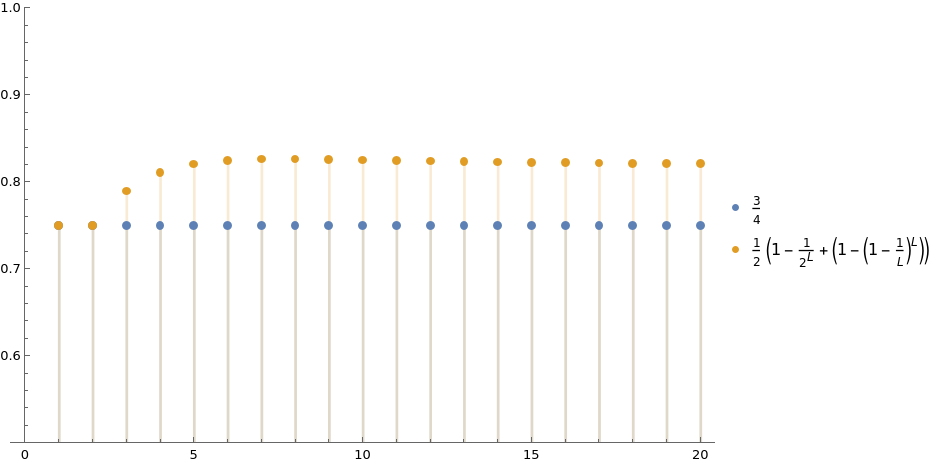
\includegraphics[width=1.25\textwidth]{figures/fig-randomrounding-bestofboth.png}
        \caption{An illustration of the last, ``magical'' inequality. Note that it does not hold for values in $(1,2)$, but, thankfully, we only need it for integers.}
        \label{fig:randomrounding:bestofboth}
    \end{figure}